\chapter{数据库设计}
采用 MariaDB 作为系统数据库存储所有系统有关的数据。数据库表和数据库表中的字段的命名规则如下。
\begin{enumerate}
	\item[(1)] 数据库表由符合相应模块功能含义的英文单词组成。
	\item[(2)] 字段命名由相应的表名称的缩写和符合字段含义的英文或拼音组成。
	\item[(3)] 命名应遵循“见名知意”的原则
\end{enumerate}
\section{数据库需求分析}
用户的需求具体体现在各种信息的提供、保存、更新和查询,这就哟啊求数据哭结构能充分满足各种信息的输入输出,收集基本数据、数据结构以及数据处理的流程。针对在线考试系统的核心流程,
通过对用户操作流程的分析,主要可以有以下所示的数据项和数据结构。
\begin{enumerate}
	\item[(1)] 用户信息。ID、昵称、密码、真实姓名、年龄、性别、生日、手机号、角色等。
	\item[(2)] 试卷表。ID、试卷名、试卷类型、试卷总分、试卷开始时间、结束时间、试题总数、建议时间、创建人、创建时间等。
	\item[(3)] 试题表。ID、试题类型、班级、分数、难度、正确答案、描述等。
	\item[(4)] 班级表。班级ID、班级名称。
	\item[(5)] 考试表。考试名、考试班级、考试描述、考试创建人、考试创建时间。
	\item[(6)] 答题表。试卷ID、试卷名字、试卷类型、答题人、得分、满分、详细描述。 
\end{enumerate}
\section{数据库概念结构设计}
根据数据库需求分析中的数据项和数据结构,设计了满足系统各个需求的实体,以及它们之间的关系.根据需求分析规划出的实体有用户实体、班级实体、试卷实体、题目实体、试题答案试题、用户回答实体。
\par
实体之间关系的E-R如图\ref{figure:er}所示
\begin{figure}[!htbp]
\centering
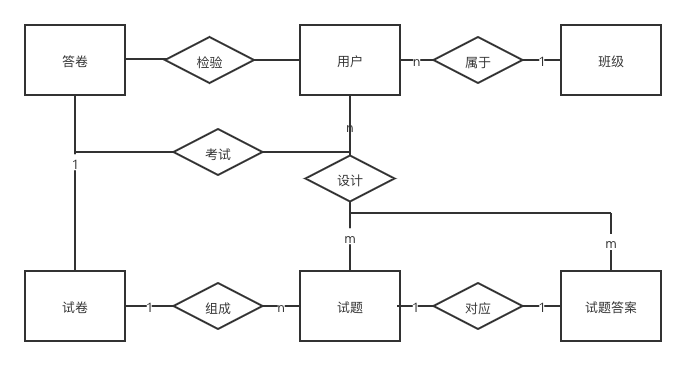
\includegraphics[width=0.6\textwidth,keepaspectratio]{data/chapter-4/er2.png}
\caption{E-R图}
\label{figure:er}
\end{figure}\section{数据库物理结构设计}
数据库物理设计阶段的任务是根据具体计算机系统和硬件等的特点,为给定的数据库模型确定合理的存储结构和存取方法。
\par
根据逻辑结构设计确定数据库中各个表及字段类型如下
\begin{enumerate}
	\item[(1)] User表,用户表用于存储用户的基本信息。如图表\ref{table:user}所示。
	\begin{table}[!htbp]
		\centering
		\begin{tabular}{|c|c|c|c|}
			\hline
			字段名 & 类型(长度) & 是否可以为空 & 说明 \\
			\hline
			ID & int(11) & PRIMARY KEY & 唯一标识 \\
			\hline
			user\_name & varchar(255) & YES & 用户名 \\
			\hline
			password & varchar(255) & YES & 密码 \\
			\hline
			real\_name & varchar(255) & YES & 真实姓名 \\
			\hline
			age & int(11) & YES	 & 年龄 \\
			\hline
			sex & int(11) & YES & 性别 \\
			\hline
			birth\_day & datetime & YES & 生日 \\
			\hline
			phone & varchar(255) & YES & 手机号 \\
			\hline
			role & int(11) & YES & 角色 \\
			\hline
			status & int(11) & YES & 状态 \\
			\hline
			image\_path & varchar(255) & YES & 头像 \\
			\hline
			create\_time & datetime & YES & 创建时间 \\
			\hline
			modify\_time & datetime & YES & 最后一次修改时间 \\
			\hline
			last\_active\_time & datetime & YES & 最后一次活动时间 \\
			\hline
			deleted & tinyint(1) & YES & 是否删除 \\
			\hline
			enabled & tinyint(1) & YES & 是否启用 \\
			\hline
			locked & tinyint(1) & YES & 是否锁定 \\
			\hline
		\end{tabular}
		\caption{用户表}
		\label{table:user}
	\end{table}
	\item[(2)] 班级表,班级表用于存储班级的基本信息。如图表\ref{table:class}所示。
	\begin{table}[!htbp]
		\centering
		\begin{tabular}{|c|c|c|c|}
			\hline
			字段名 & 类型(长度) & 是否可以为空 & 说明 \\
			\hline
			ID & int(11) & PRIMARY KEY & 唯一标识 \\
			\hline
			name & varchar(255) & YES & 班级名 \\
			\hline
			deleted & tinyint(1) & YES & 是否删除 \\
			\hline
		\end{tabular}
		\caption{班级表}
		\label{table:class}
	\end{table}
	\item[(3)] 试题表,试题表主要用于存储实体的基本信息,主要有ID、试题类型、班级、分数、难度、正确答案、描述等。如图表\ref{table:question}所示。
	\begin{table}[!htbp]
		\centering
		\begin{tabular}{|c|c|c|c|}
			\hline
			字段名 & 类型(长度) & 是否可以为空 & 说明 \\
			\hline
			ID & int(11) & PRIMARY KEY & 唯一标识 \\
			\hline
			score & int(11) & YES & 分数 \\
			\hline
			grade\_level & int(11) & YES & 班级 \\
			\hline
			difficult & int(11) & YES & 难度 \\
			\hline
			correct & text & YES & 正确答案 \\
			\hline
			info\_text\_content\_id & int(11) & YES & 上下文唯一标识符 \\
			\hline
			create\_user & int(11) & YES & 创建人 \\
			\hline
			status & int(11) & YES & 状态 \\
			\hline
			create\_time & datetime & YES & 创建时间 \\
			\hline
			deleted & tinyint(1) & YES & 是否删除 \\
			\hline
		\end{tabular}
		\caption{题目表}
		\label{table:question}
	\end{table}
	\item[(4)] 试卷表,试卷表主要用于存储试卷实体的基本信息。试卷ID、试卷名称和内容。如图表\ref{table:paper}所示。
	\begin{table}[!htbp]
		\centering
		\begin{tabular}{|c|c|c|c|}
			\hline
			字段名 & 类型(长度) & 是否可以为空 & 说明 \\
			\hline
			ID & int(11) & PRIMARY KEY & 唯一标识 \\
			\hline
			name & varchar(255) & YES & 名字 \\
			\hline
			paper\_type & int(11) & YES & 试卷类型 \\
			\hline
			grade\_level & int(11) & YES & 班级 \\
			\hline
			score & int(11) & YES & 分数 \\
			\hline
			question\_count & int(11) & YES & 问题数 \\
			\hline
			suggest\_time & int(11) & YES & 建议时间 \\
			\hline
			limit\_start\_time & datetime & YES & 开始时间 \\
			\hline
			limit\_end\_time & datetime & YES & 结束时间 \\
			\hline
			frame\_text\_content\_id & int(11) & YES & 内容ID \\
			\hline
			create\_user & int(11) & YES & 创建人 \\
			\hline
			create\_time & datetime & YES & 创建时间 \\
			\hline
			deleted & bit(1) & YES & 是否删除 \\
			\hline
			task\_exam\_id & int(11) & YES & 考试ID \\
			\hline
		\end{tabular}
		\caption{试卷表}
		\label{table:paper}
	\end{table}
	\item[(5)] 考试表,考试表用于存储考试的基本信心。主要包括考试名、考试班级、考试描述、考试创建人、考试创建时间。如图表\ref{table:exam}所示。
	\begin{table}[!htbp]
		\centering
		\begin{tabular}{|c|c|c|c|}
			\hline
			字段名 & 类型(长度) & 是否可以为空 & 说明 \\
			\hline
			ID & int(11) & PRIMARY KEY & 唯一标识 \\
			\hline
			title & varchar(255) & YES & 标题 \\
			\hline
			grade\_level & int(11) & YES & 班级 \\
			\hline
			frame\_text\_content\_id & int(11) & YES & 内容ID \\
			\hline
			create\_user & int(11) & YES & 创建人 \\
			\hline
			create\_time & datetime & YES & 创建时间 \\
			\hline
			deleted & bit(1) & YES & 是否删除 \\
			\hline
			create\_user\_name & varchar(255) & YES & 创建人姓名 \\
			\hline
		\end{tabular}
		\caption{考试表}
		\label{table:exam}
	\end{table}
	\item[(6)] 答题表,答题表用于存储答题的基本信息。主要包括试卷ID、试卷名字、试卷类型、答题人、得分、满分、详细描述。 如图表\ref{table:dati}所示。
	\begin{table}[!htbp]
		\centering
		\begin{tabular}{|c|c|c|c|}
			\hline
			字段名 & 类型(长度) & 是否可以为空 & 说明 \\
			\hline
			ID & int(11) & PRIMARY KEY & 唯一标识 \\
			\hline
			question\_id & int(11) & YES & 问题的唯一标识 \\
			\hline
			exam\_paper\_id & int(11) & YES & 试卷的唯一标识 \\
			\hline
			exam\_paper\_answer\_id & int(11) & YES & 试卷答案的唯一标识 \\
			\hline
			question\_type & int(11) & YES & 问题类型 \\
			\hline
			customer\_score & int(11) & YES & 用户分数 \\
			\hline
			question\_score & int(11) & YES & 问题分数 \\
			\hline
			question\_text\_content\_id & int(11) & YES & 问题内容ID \\
			\hline
			answer & varchar(255) & YES	 & 答案 \\
			\hline
			text\_content\_id & int(11) & YES & 描述ID \\
			\hline
			do\_right & bit(1) & YES & 是否正确 \\
			\hline
			create\_user & int(11) & YES & 创建人 \\
			\hline
			create\_time & datetime & YES & 创建时间 \\
			\hline
		\end{tabular}
		\caption{考试表}
		\label{table:dati}
	\end{table}
\end{enumerate}
